% Por hacer:
% Mejorar los dibujos que se tomaron del Spivak (crear un dibujo tikz)

\section{Integrales de Riemann}

En este curso se desarrollará la idea de integral de Riemann para funciones definidas en un intervalo $[a,b]$. Y será muy útil para desarrollar la noción del cálculo del volumen y área de los cuerpos geométricos.

Por ahora, intentaremos definir el área de las regiones limitadas por:

\begin{itemize}
    \item El eje horizontal.
    \item Las verticales por $(a,0)$ y $(b,0)$.
    \item La gráfica de una función $f$ tal que $f(x) \geq 0$ para todo $x$ de $[a,b]$.
\end{itemize}

\begin{figure}[h]
    \centering
    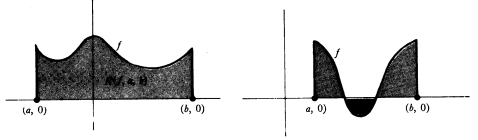
\includegraphics[scale=0.8]{img/cap1.png}
    \caption{\footnotesize En esta figura se pueden ver los puntos descritos. Si $f$ es una función dibujada como en la segunda figura, la integral representará la diferencia entre las regiones por encima de la línea horizontal y por debajo de la misma.}
\end{figure}

Eventualmente esta área recibirá el nombre de \textbf{integral de $f$ sobre $[a,b]$}. Pero en un principio, hemos de desarrollar la idea de \textbf{partición} de un intervalo.

\subsection{Partición de un intervalo}

\begin{defn}
Sea $a<b$, recibe el nombre de \ul{partición} del intervalo $I = [a,b]$ toda colección finita de puntos de $I$ de los cuales uno es $a$ y otro es $b$. Los puntos de una partición pueden ser numerados $x_0, \dots, x_n$, de manera que

\[
a = x_0 < x_1 < \dots < x_{n-1} < x_n = b
\]
\end{defn}

Entonces en líneas generales, la partición nos va a permitir representar a un intervalo como una unión de intervalos más pequeños (todos cerrados)\marginfootnote{O, dicho de una manera más concreta $[a,b] = \bigcup_{j=1}^n [x_{j-1},x_j]$}.

En un mismo intervalo se pueden considerar muchos tipos de particiones, pero entre todas ellas, la que más nos va a interesar es la \ul{partición canónica}\marginfootnote{Esto no es más que tomar la distancia del intervalo y dividirla entre algún $n \in \N$ para hallar la longitud que tomará cada subintervalo (todos tendrán la misma longitud).}:

\[
x_j = a + \frac{j}{n}(b-a), \quad j = 0 \dots n, \quad n \in \N
\]

Un ejemplo de una partición canónica en un intervalo bien podría ser:

\begin{center}
    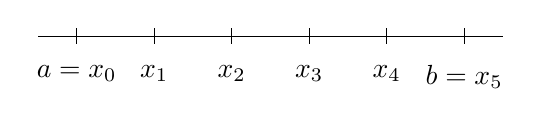
\begin{tikzpicture}[x=70]
       \draw (-0.2,0) -- (2.2,0);      
       \draw (0, 0) node[below=7pt] {$a=x_0$};
       \draw[] (0,-0.1) -- (0,0.1);
       \draw (0.4, 0) node[below=7pt] {$x_1$};
       \draw[] (0.4,-0.1) -- (0.4,0.1);
       \draw (0.8, 0) node[below=7pt] {$x_2$};
       \draw[] (0.8,-0.1) -- (0.8,0.1);
       \draw (1.2, 0) node[below=7pt] {$x_3$};
       \draw[] (1.2,-0.1) -- (1.2,0.1);
       \draw (1.6, 0) node[below=7pt] {$x_4$};       
       \draw[] (1.6,-0.1) -- (1.6,0.1);
       \draw (2, 0) node[below=7pt] {$b=x_5$};
       \draw[] (2,-0.1) -- (2,0.1);
    \end{tikzpicture}
\end{center}

\begin{nota}
    Tomaremos $\Pa([a,b])$ como el conjunto de particiones del intervalo $[a,b]$.
\end{nota} 

\begin{nota}
    Como se consideró anteriormente, el intervalo canónico $[a,b]$ puede considerarse como

    \[
    [a,b] = \bigcup_{j=1}^n I_j \quad \text{donde} \quad I_j = [x_{j-1}, x_j]
    \]
    
    \noindent la longitud de cada subintervalo es
    
    \[
    |I_j| = \frac{b-a}{n}
    \]
    
    \noindent y cada punto estará determinado por
    
    \[
    x_j = a + \frac{j}{n}(b-a)
    \]
\end{nota} 

\begin{defn}
    En $\Pa([a,b])$ se puede establecer una relación de orden: Sean $P_1$ y $P_2$ particiones de $[a,b]$, entonces diremos que $P_1 < P_2$ o que $P_2$ es \ul{refinamiento} de $P_1$ si y solamente si $P_1 \subset P_2$\marginfootnote{O dicho de otra manera, $P_2$ tiene más puntos que $P_1$, e incluye todos los de $P_1$. Esta es una relación de orden, y se puede verificar.}.\marginnote{\ejem Un ejemplo de refinamiento es el siguiente:

    \begin{gather*}
        P_1 = \{ a, x_1, x_2, x_3 \} \\
        P_2 = \{ a, x_1, y_1 x_2, y_2 x_3, y_3, b\}
    \end{gather*}
    
    \noindent tenemos que $P_2$ refina a $P_1$.}
\end{defn} 

\begin{pro}
    Sean $P_1, P_2 \in \Pa([a,b])$ entonces existe una partición $P_3 \in \Pa$ tal que $P_1 < P_3$ y $P_2 < P_3$.
\end{pro}

\begin{proof}
    Sean $P_1$ y $P_2$ tales que
    
    \begin{gather*}
        P_1 = \{ x_j \}_{j=0}^n \\
        P_2 = \{ x_k \}_{k=0}^m
    \end{gather*}
    
    \noindent definamos entonces a $P_3$ como
    
    \[
    P_3 = P_1 \cup P_2
    \]
    
    \noindent entonces, como $P_3$ es la unión, nos queda que $P_1 \subset P_3$ y $P_2 \subset P_3$. Y así queda demostrado.
\end{proof}

Ahora, para cualquier partición, si consideramos una función cualquiera $f$, entonces sobre el primer intervalo $[x_0, x_1]$, la función $f$ tendrá el valor mínimo $m_1$ y el valor máximo $M_1$. Análogamente, sea $m_i$ el valor mínimo y $M_i$ el valor máximo de $f$ sobre el intervalo $i$-ésimo. La suma

\[
L(f, P) = \sum_{j=1}^n m_j(x_j - x_{j-1})
\]

\noindent representa el área total de los rectángulos que están dentro de la región, mientras que la suma

\[
U(f, P) = \sum_{j=1}^n M_j(x_j - x_{j-1})
\]

\noindent representa el área total de los rectángulos que contienen la región.

\begin{figure}[h]
    \centering
    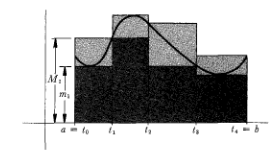
\includegraphics[scale=0.8]{img/cap2.png}
    \label{fig:areamM}
\end{figure}

Si el área buscada es $A$, entonces $A$ debe satisfacer

\[
L(f, P) \leq A \quad \text{y} \quad A \leq U(f, P)
\]

\noindent de forma más concreta, podemos enunciar la siguiente definición.

\begin{defn}
    Supongamos que $f$ es acotada sobre $[a,b]$ y $P = \{ x_0, \dots, x_n \}$ es una partición de $[a,b]$. Sea

    \begin{gather*}
        m_i(f, I_j) = \inf \{ f(x) : x_{j-1} \leq x \leq x_j \} \\
        M(f, I_j) = \sup \{ f(x) : x_{j-1} \leq x \leq x_j \}
    \end{gather*}
    
    La \ul{suma inferior} de $f$ para $P$, designada por $L(f,P)$ se define poniendo
    
    \[
    L(f, P) = \sum_{j=1}^n m_j(f, I_j)|I_j|
    \]
    
    La \ul{suma superior} de $f$ para $P$, designada por $L(f,P)$ se define poniendo
    
    \[
    U(f, P) = \sum_{j=1}^n M_j(f, I_j)|I_j|
    \]
\end{defn}

\begin{teo}\marginfootnote{Este teorema junto a su demostración aparece de una forma un poco más desglosada en el Spivak, capítulo 13.}
    Sea $f: [a,b] \rightarrow \R$ acotada. Sean $P_1$ y $P_2$ dos particiones en $[a,b]$ tales que $P_1 < P_2$, entonces se cumple

    \[
    L(f, P_1) \leq L(f, P_2) \leq U(f, P_2) \leq U(f, P_1)
    \]
\end{teo}

\begin{proof}
    Supongamos primero que $P_2$ es refinamiento de $P_1$ apenas por un punto que llamaremos $z_1$, es decir
    
    \[
    P_1 = \{ x_j \}_{j=0}^n \quad P_2 = P_1 \cup \{ z_1 \}
    \]
    
    A los intervalos de $P_1$ los representaremos con la variable $I_j$ ($j = 1, \dots, n$), y el intervalo donde está colocado $z_1$ en la partición $P_2$, lo llamaremos $I_{j_0}$. Visualmente, tendremos lo siguiente:
    
    \begin{center}
        \begin{tikzpicture}[x=70]
           \draw (-0.2,0) -- (2.2,0);      
           \draw (0, 0) node[below=7pt] {$a$};
           \draw[] (0,-0.1) -- (0,0.1);
           \draw[] (0.4,-0.1) -- (0.4,0.1);
           \draw[] (0.8,-0.1) -- (0.8,0.1);
           \draw (1, 0) node[below=7pt] {\ul{$z_1$}};
           \draw[] (1,-0.1) -- (1,0.1);
           \draw[decorate, decoration = {calligraphic brace, raise=5pt, amplitude=5pt}] (0.8,0.1) --  (1.2,0.1) node[pos=0.5,above=10pt,black]{$I_{j_0}$};
           \draw[] (1.2,-0.1) -- (1.2,0.1);
           \draw[] (1.6,-0.1) -- (1.6,0.1);
           \draw (2, 0) node[below=7pt] {$b$};
           \draw[] (2,-0.1) -- (2,0.1);
        \end{tikzpicture}
    \end{center}\marginnote{Aquí está representado $P_2$.}
    
    $I_{j_0}$ será equivalente al intervalo $[x_{j_0-1}, x_{j_0}]$. Por otro lado, sabemos por definición que
    
    \[
    L(f, P_1) = \sum_{j=1}^n m(f, I_j)|I_j|
    \]
    
    \noindent esta suma la podemos expresar de la siguiente manera:
    
    \[
    \sum_{j=1}^n m(f, I_j)|I_j| = \sum_{j \neq j_0} m(f, I_j)|I_j| + m(f, I_{j_0})|I_{j_0}|
    \]
    
    \noindent como $m(f,I_{j_0})$ se refiere al ínfimo de la función cuando $f$ está sobre el intervalo $I_{j_0}$, entonces como $I_{j_0} \supset [x_{j_0}-1,z_1]$, tenemos que\marginfootnote{Aquí se hace uso del siguiente teorema:
    \teo Si $A \subset B$ entonces $\inf A \geq \inf B$.
    \begin{proof} Si $m = \inf B$, entonces $m \leq b, \forall b \in B$. Como $A \subset B$, entonces $m \leq a, \forall a \in A$, y esto implica que $m \leq \inf A$. De esta forma, queda demostrado. \end{proof} }
    
    \[
    m(f, I_{j_0}) \leq m(f, [x_{j_0-1},z_1])
    \]
    
    \noindent de forma análoga, tenemos que
    
    \[
    m(f, I_{j_0}) \leq m(f, [z_1, x_{j_0}])
    \]
    
    \noindent de esta forma, tenemos que
    
    \begin{align*}
        m(f, I_{j_0})&|I_{j_0}| = m(f, I_{j_0})|z_1 - x_{j_0-1}| + m(f, I_{j_0})|x_{j_0} - z_1| \\
        &\leq m(f, [x_{j_0-1},z_1])|z_1 - x_{j_0-1}| + m(f, [z_1, x_{j_0}])|x_{j_0} - z_1|
    \end{align*}
    
    Ahora, nos queda
    
    \begin{align*}
        L(f, P_1) &= \sum_{j \neq j_0} m(f, I_j)|I_j| + m(f, I_{j_0})|I_{j_0}| \\
        &\leq \sum_{j \neq j_0} m(f, I_j)|I_j| + m(f, [x_{j_0-1},z_1])|z_1 - x_{j_0-1}| + m(f, [z_1, x_{j_0}])|x_{j_0} - z_1| \\
        &= L(f, P_2)
    \end{align*}
    
    \noindent de esta forma $L(f,P_1) \leq L(f, P_2)$ cuando $P_1 < P_2$ por un punto de diferencia. Esta demostración se puede utilizar para un contexto más general:
    
    Sea $P_1 = \{x_j\}_{j=0}^n$ y $P_2 = \{y_k\}_{k=0}^m$, como $P_1 < P_2$, todo punto de $P_1$ pertenece a $P_2$, y en $P_2$ habrán valores que no pertenecen a $P_1$. Entonces, sea $P_2 \smallsetminus P_1 = \{ z_j \}_{j=0}^{m-n}$ (suponiendo que $m > n$). Entonces, procediendo de manera inductiva repetimos el razonamiento anterior para $P_2 = P_1 \cup \{z_1, z_2\}$ y así de forma sucesiva hasta abarcar todos los puntos que constituyen a $P_2 \smallsetminus P_1$.
    
    De esta forma, ya tenemos demostrada una parte de la desigualdad.
    
    Por definición sabemos que $L(f, P_2) \leq U(f,P_2)$, por lo que esta parte es trivial.
    
    Nos queda solamente demostrar que $U(f, P_2) \leq U(f, P_1)$: El procedimiento es análogo a la desigualdad anterior, entonces como\marginfootnote{Aplicamos un teorema análogo al de la nota anterior:
    
    \begin{teo}
    Si $A \subset B$ entonces $\sup A \leq \sup B$.
    \end{teo}
    
    \begin{proof}
    Si $M = \sup B$, entonces $M \geq b, \forall b \in B$. Como $A \subset B$, entonces $M \geq a, \forall a \in A$, y esto implica que $M \geq \sup A$. De esta forma, queda demostrado.
    \end{proof}}
    
    \begin{align*}
        M(f, I_{j_0})&|I_{j_0}| = M(f, I_{j_0})|z_1 - x_{j_0-1}| + M(f, I_{j_0})|x_{j_0} - z_1| \\
        &\geq M(f, [x_{j_0-1},z_1])|z_1 - x_{j_0-1}| + M(f, [z_1, x_{j_0}])|x_{j_0} - z_1|
    \end{align*}
    
    \noindent nos queda que
    
    \begin{align*}
        U(f, P_1) &= \sum_{j \neq j_0} M(f, I_j)|I_j| + M(f, I_{j_0})|I_{j_0}| \\
        &\geq \sum_{j \neq j_0} M(f, I_j)|I_j| + M(f, [x_{j_0-1},z_1])|z_1 - x_{j_0-1}| + M(f, [z_1, x_{j_0}])|x_{j_0} - z_1| \\
        &= U(f, P_2)
    \end{align*}
    
    Igual que para la desigualdad anterior, aplicamos un razonamiento inductivo para el caso general.
    
    Finalmente, tenemos que
    
    \[
    L(f, P_1) \leq L(f, P_2) \leq U(f, P_2) \leq U(f, P_1)
    \]
    
    \noindent y queda demostrado el teorema.
\end{proof}

\subsection{Funciones integrables en el sentido de Riemann}

Es importante resaltar que a medida que vayamos refinando la partición, las sumas superiores van a ir constituyendose en una sucesión decreciente, es decir, las área de los rectángulos que las conforman van a irse acercando a la función $f$. Lo mismo ocurre con las sumas inferiores, solo que las áreas van a constituir una sucesión creciente.

Esto nos da pie a la siguiente definición.

\begin{defn}
    Una función $f$ acotada sobre $[a,b]$ es \ul{integrable (en el sentido de Riemann)} sobre $[a,b]$ si y solamente si
    
    \[
    \sup_P L(f,P) = \inf_P U(f,P)
    \]
\end{defn}

Ahora, lo interesante es hacernos la siguiente pregunta:

\begin{pre}
    ¿Cómo debe ser $f$ para que sea integrable?
\end{pre}